\documentclass[manuscript,review,anonymous]{acmart}
\usepackage{booktabs}
\usepackage{graphicx}
\setcopyright{none}
\settopmatter{printacmref=false}
\acmDOI{}
\acmISBN{}
\title{Separating Calibration from Feature Compression in Longitudinal Alzheimer's Microbiome Classification}
\begin{document}
\begin{abstract}
Repeated visits and correlated clinical covariates complicate evaluation of microbiome classifiers. We audit an Alzheimer's cohort containing 335 visits from 102 subjects using paired subject-level folds, conformal prediction sets, compositional sensitivity analysis and subject-resampled intervals. Full and compact XGBoost predictors are compared with and without calibration using identical fitting, calibration and test subjects. Class-conditional calibration and trivial baselines expose the trade-off between coverage and abstention. We provide executable evaluation audits rather than a new classifier or conformal theorem. All numerical results below are generated from recorded experiments. An exploratory genus-only comparison on AlzBiom yielded AUROC 0.561.
\end{abstract}
\maketitle
\section{Problem and scope}
The ADAM-1 framework integrates microbiome and clinical variables for Alzheimer's classification \cite{huang}. Its bundled cohort contains repeated visits with constant diagnosis per participant. Random visit splitting can let subject identity influence test performance. Our study evaluates this tabular cohort, not the original paper's complete language-model reasoning workflow.

We ask how participant separation changes apparent discrimination, how much prediction-set coverage costs in abstention, and whether compression changes these results when calibration is held fixed. We do not assume compression improves coverage or that predictive clinical covariates identify a microbial mechanism.

\section{Related work and contribution}
Dudek et al.\ review weaknesses in microbiome machine-learning practices \cite{dudek}. Du et al.\ evaluate subject-stratified random forests on longitudinal HMP2 data \cite{hmp2}. CRC-TrustBench combines leakage-aware evaluation and reliability assessment across colorectal-cancer studies and countries \cite{crc}. Neither leakage audits nor microbiome calibration benchmarks are new. Split conformal prediction is established \cite{angelopoulos}.

Our contribution is an executable application and correction of these principles for this ADAM cohort: paired full/compact ablations, fitting-subject and feature-selection audit trails, a corrected calibration unit, and subject-balanced coverage/abstention reporting. We make no priority claim, new-algorithm claim or acceptance guarantee.

\section{Data and protocol}
The bundled table contains 940 taxonomy-matched species and 104 other predictors after excluding sample and subject IDs, diagnosis, date, age and other-dementia metadata. Coarse age category and visit day remain and are audited. Invalid IDs, duplicate samples, changing or nonbinary labels, and nonfinite features are rejected. Feature missingness follows the existing zero-fill convention, a limitation particularly for clinical fields.

For seeds 42--71, unique subjects are partitioned into five test folds. Each remaining subject pool is partitioned into fitting and calibration subsets, approximately two thirds and one third, independently of outcomes. Full and compact models share exact partitions. Compact models retain 96 species selected by prevalence among fitting subjects, plus 104 other predictors. Selection is rerun inside each fold. A regression test perturbs all nonfitting observations and verifies selection invariance.

XGBoost uses 100 trees, depth 6, learning rate 0.1, row and column subsampling 0.8, one thread and training-class weighting. Model seeds follow split seeds. A separate nested-CV sensitivity experiment uses seed 42, five stratified subject outer folds, three inner folds, and five Optuna trials over depth, tree count and learning rate. Compact selection is rerun inside every inner fitting partition. This small search budget is not evidence of global optimality.

\section{Calibration and statistical analysis}
With fitted visit probabilities $p_{ij}$ and subject diagnosis $y_i$, define
\[
r_{ij}=1-\widehat P(Y=y_i\mid x_{ij}),\qquad s_i=\max_j r_{ij}.
\]
For $n$ calibration subjects, use order statistic $k=\lceil(n+1)(1-\alpha)\rceil$, or threshold 1 when $k>n$. Include test label $c$ when $1-\widehat P(c\mid x_{ij})\leq q$. Subject coverage requires the true label at every observed visit. This corrects the supplied patch's pooling of visit calibration scores despite subject-disjoint splitting.

Mondrian thresholds $q_c$ use only calibration subjects of class $c$. Small or absent classes receive conservative inclusion. This targets class-conditional simultaneous coverage under within-class exchangeability; empirical equality and cross-cohort validity do not follow. Nursing-home dependence and different visit patterns may violate exchangeability.

Forced choice, full/compact subject calibration, and full/compact Mondrian methods use paired fits. The always-both-label reference has perfect coverage and no singleton predictions. The class-prior baseline estimates prevalence from fitting subjects and predicts the majority class. Risk--coverage curves vary $\alpha$ over 0.05, 0.10, 0.20, 0.30 and 0.40; horizontal coverage means singleton acceptance and risk means singleton error, with subjects weighted equally.

Intervals use 1,000 bootstrap draws of subjects retaining all their repeats. They are conditional on fitted out-of-fold models and omit refitting uncertainty. Artifact AUROC intervals use probabilities averaged over visits and repeats; per-seed AUROCs are stored separately. Repeated folds are not independent cohorts. Paired coverage differences use the same resampled subjects.

The permutation test reassigns labels at subject level, reconstructs stratified folds and refits the default full model for 199 permutations. Its plus-one $p$-value has resolution 0.005. This is an unadjusted global-exchangeability test, separate from tuning and not conditional on clinical covariates or nursing home.

\section{Results}
\begin{table}
\caption{Subject-balanced results over 30 repeated five-fold partitions. Coverage intervals resample subjects, conditional on fitted predictions.}
\centering\small
\begin{tabular}{lrrr}
\toprule
Method & Subject coverage [95\% CI] & Singleton & AD coverage\\
\midrule
class\_prior & 0.627 [0.529, 0.716] & 1.000 & 0.000\\
always\_both & 1.000 [1.000, 1.000] & 0.000 & 1.000\\
full\_forced & 0.570 [0.512, 0.631] & 1.000 & 0.447\\
full\_subject & 0.931 [0.900, 0.960] & 0.222 & 0.882\\
full\_mondrian & 0.929 [0.898, 0.958] & 0.201 & 0.934\\
compact\_forced & 0.568 [0.509, 0.633] & 1.000 & 0.414\\
compact\_subject & 0.925 [0.894, 0.956] & 0.226 & 0.872\\
compact\_mondrian & 0.923 [0.895, 0.950] & 0.199 & 0.927\\
clr\_full\_subject & 0.925 [0.893, 0.952] & 0.215 & 0.870\\
\bottomrule
\end{tabular}
\end{table}
The unadjusted subject permutation test yielded AUROC 0.772 and $p=0.005$ over 199 permutations.
Nested full XGBoost subject AUROC was 0.725 (one outer seed, five trials per fold).
Nested compact XGBoost subject AUROC was 0.751 (one outer seed, five trials per fold).
full\_subject\_minus\_full\_forced: coverage difference 0.361, bootstrap interval [0.315, 0.407].
compact\_subject\_minus\_full\_subject: coverage difference -0.006, bootstrap interval [-0.013, 0.001].
compact\_forced\_minus\_full\_forced: coverage difference -0.002, bootstrap interval [-0.018, 0.013].
full\_mondrian\_minus\_full\_subject: coverage difference -0.002, bootstrap interval [-0.016, 0.013].
Intervals and point estimates must be interpreted jointly with singleton acceptance; perfect coverage alone is achieved by the always-both baseline.
Across 5 held-out folds with 30 training-subject bootstrap refits each, mean pairwise Jaccard similarity of the top 20 features was 0.244 (fold range 0.220 to 0.260).

\begin{figure}
\centering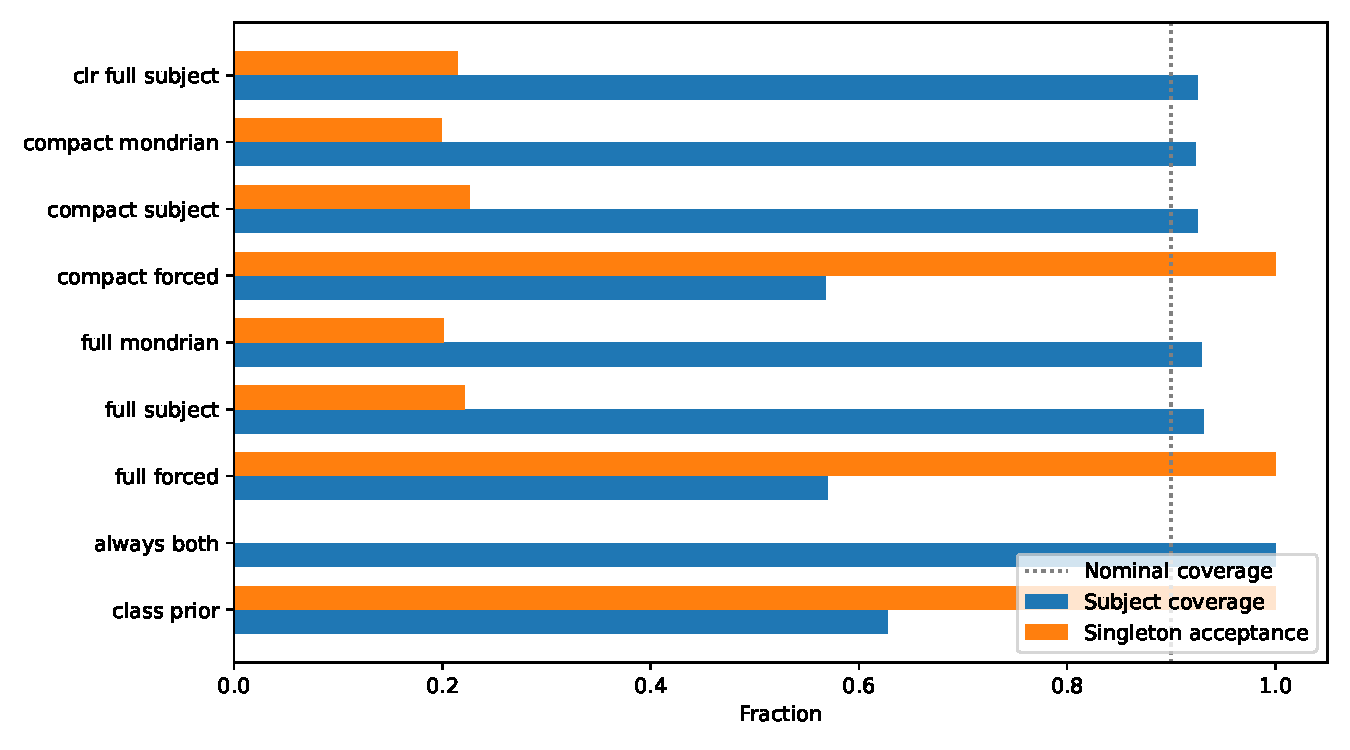
\includegraphics[width=.95\linewidth]{figures/coverage.pdf}
\caption{Subject simultaneous coverage and singleton acceptance from the repeated-fold artifact; bootstrap intervals appear in the table.}
\Description{Comparison of coverage and singleton acceptance for paired methods and trivial baselines.}
\end{figure}
\begin{figure}
\centering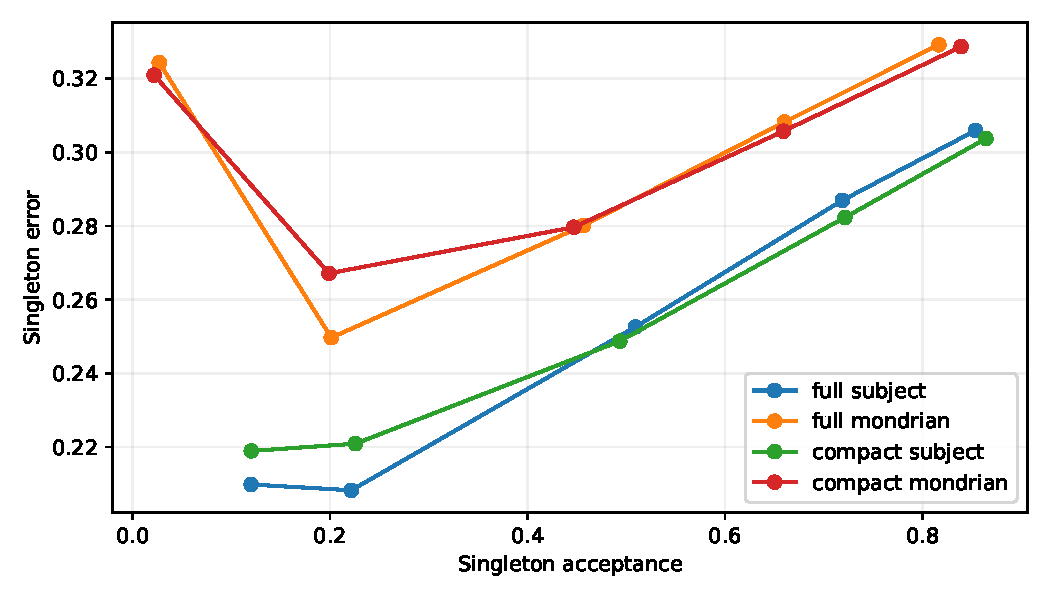
\includegraphics[width=.85\linewidth]{figures/risk_coverage.pdf}
\caption{Singleton error versus singleton acceptance at prespecified conformal levels. These descriptive curves do not select thresholds on test labels.}
\Description{Risk and acceptance curves for full and compact subject and Mondrian calibration.}
\end{figure}

\section{Composition, proxies and external validation}
CLR sensitivity closes each abundance vector, adds a fixed $10^{-6}$ pseudocount, and centers log abundances within sample. Clinical columns remain unchanged. Negative abundances and all-zero compositions are rejected. No transform parameter is selected on test labels.

Proxy ablations remove age category/day, frailty/nutrition, and a recorded medication subset in separate grouped-CV runs. They assess predictive dependence, not causality or complete confounding adjustment. Medication use can encode diagnostic treatment. For the explanation stability audit, each bootstrap draw resamples training subjects with all their visits. Each refitted tree model explains the same held-out subjects in its fold. We rank features by absolute SHAP contribution, averaging visits within subject before averaging across subjects. Within each fold we compare all pairs of top-20 sets using intersection size divided by union size. This measures sensitivity to the training sample under one outer split and one model seed. Correlated features may substitute for one another.

In an exploratory external comparison, a genus-only logistic model used 97 genera shared with the AlzBiom archive (PRJEB47976, Laske et al., doi:10.3389/fnins.2022.792996). We aggregated 357 ADAM species columns, renormalized each sample over the shared genera, took square roots, and averaged transformed visits within each ADAM participant. The L2 penalty used fixed inverse strength $C=1$ throughout. All fitting used 102 ADAM participants. Both published AlzBiom partitions were scored together with frozen coefficients.

Across 75 cases and 100 controls, AUROC was 0.561 (95\% stratified bootstrap interval 0.474--0.647, conditional on the fitted model). In 2,000 additional replicates independently resampling ADAM participants with refitting and AlzBiom records within class, the percentile interval was 0.455--0.656. Both intervals retain the shared feature schema and assume independence of distinct external records. Discrimination above chance was undetectable at this precision. Brier scores were 0.24793 for the model, 0.24804 for ADAM prevalence and 0.24490 for the retrospective target-prevalence oracle. Source and target case fractions were 37.3\% and 42.9\%. The calibration intercept with unit slope was 0.329; jointly estimated intercept and slope were 0.607 and 1.453. Calibration fits were descriptive and did not alter predictions.

Profiling pipelines, taxonomy synonyms, normalization, ascertainment, diet and geography may contribute to differences between cohorts. This analysis cannot attribute the result to any one factor. The interval allows modest discrimination. In a subsequent exploratory comparison, five-fold stratified cross-validation among ADAM participants minimized Brier score over inverse penalties 0.01, 0.1, 1, 10 and 100. It selected the original value of 1 and reproduced the same external scores. Independent-cohort evaluation of the species-plus-clinical model and its conformal coverage remains outstanding.

\section{Limitations and reproducibility}
This is one small retrospective cohort; all seeds reuse 102 subjects. Group separation does not remove acquisition, nursing-home or treatment effects. Conditional intervals omit refitting variability. Nested tuning uses one seed and a small budget; proxy ablations are not causal adjustment. The original LLM pipeline was not rerun. External validity, prospective calibration and clinical utility remain unestablished.

Run \texttt{python -m app.research.rigor} and \texttt{python -m app.research.repeated} in \texttt{backend/}, then \texttt{python -m app.research.heldout\_stability}, followed by \texttt{python manuscript/generate.py} at repository root. Artifacts record versions, seeds, matrix/label/group/feature hashes and fitting-subject selections. Synthetic test fixtures are not experimental results. Patch-supplied measurements were replaced by executed measurements. The software's optional-storage mode preserves file-backed research during a DB outage; it does not restore a missing database. This manuscript is a research draft, not a clinically validated product.
\bibliographystyle{ACM-Reference-Format}
\bibliography{references}
\end{document}
